\usepackage{epsfig, supertabular, makeidx}

\usepackage{amsmath, amssymb}

% Package to add Bibliography and Index to TOC
% but not the TOC itself :-)
\usepackage[nottoc]{tocbibind}

\usepackage{hangcaption}
\usepackage{subfigure}
\usepackage{color}

% Needed for sideways
\usepackage{rotating}

% Packages needed for the cover page
\usepackage{calc, epsfig, chngpage}
\input{pstricks}\input{pst-node}% ***************** llnlCoverPage.tex ********************************************************************************
% This file defines the following commands for generating the
% front and back cover pages:
%
%     \makeLLNLCover{UCRL}{Title}{Authors}{Journal}{Date}{hShift}{vShift}
%  and
%     \makeLLNLBackCover
%      
% where
%
%  UCRL: The UCRL (6 digit) number (which you probably won't know before the document 
%        is released so just make up a number)
%  Title: title of the article
%  Authors: Authors separated by \\
%  Journal: The journal name
%  Date : the date
%  hShift,vShift : horizontal and vertical shifts to apply to the title page to position it correctly (since
%                  the automatic positioning may not work)
%
% Here is an example:
%  \makeLLNLCover{123456}{An adaptive numerical method for high-speed reactive flows}{William D. Henshaw\\%
%   Donald W. Schwendeman}{Journal of Computational Physics}{January 1, 2003}{0in}{0in}
% 
% *****************************************************************************************************************
% 
\newcommand{\setPageForLLNLCover}[2]{%
\newlength{\textwidthOld}%
\setlength{\textwidthOld}{\textwidth}%
\newlength{\textheightOld}%
\setlength{\textheightOld}{\textheight}%
\newlength{\topmarginOld}%
\setlength{\topmarginOld}{\topmargin}%
\newlength{\textwidthNew}%
\setlength{\textwidthNew}{6.5in}%
\newlength{\textheightNew}%
\setlength{\textheightNew}{9.5in}%
\newlength{\oddsidemarginNew}%
\newlength{\topmarginNew}%
\setlength{\oddsidemarginNew}{(\paperwidth-\textwidthNew)/2 - 1in + #1}%
\setlength{\topmarginNew}{(\paperheight-\textheightNew -\headheight-\headsep-\footskip)/2 - 1in +1.cm + #2}%
\newlength{\oddsidemarginOld}%
\setlength{\oddsidemarginOld}{\oddsidemargin}%
\changepage{\textheightNew-\textheightOld}{\textwidthNew-\textwidthOld}{\oddsidemarginNew-\oddsidemarginOld}{\oddsidemarginNew-\oddsidemarginOld}{}{\topmarginNew-\topmarginOld}{}{}{}%
}%
\newcommand{\setPageForLLNLBackCover}{%
\changepage{\textheightNew-\textheightOld}{\textwidthNew-\textwidthOld}{\oddsidemarginNew-\oddsidemarginOld}{\oddsidemarginNew-\oddsidemarginOld}{}{\topmarginNew-\topmarginOld}{}{}{}%
}%
\newcommand{\resetPageFromLLNLCover}{%
\changepage{-\textheightNew+\textheightOld}{-\textwidthNew+\textwidthOld}{-\oddsidemarginNew+\oddsidemarginOld}{-\oddsidemarginNew+\oddsidemarginOld}{}{-\topmarginNew+\topmarginOld}{}{}{}%
}%
% *************************************************************************************


% *************************************************************************************
\newcommand{\makeLLNLCover}[6]{%
\setPageForLLNLCover{#5}{#6}%
\thispagestyle{empty}% no number of this page
\newcommand{\logoWidth}{1.65in}% 
\psset{xunit=1.cm,yunit=1.cm,runit=1.cm}%
\begin{pspicture}(0,0)(17,24.)
% turn on the grid for placement
% \psgrid[subgriddiv=2]
\rput(2.3,11.5){\epsfig{file=Logo_for_papers.ps,width=\logoWidth}}
\rput(11.2,23.){\parbox{12.0cm}{\large\bf%
\begin{flushright}
Preprint \\
UCRL-MA-#1
\end{flushright}
}}
\rput(10.5,18){\parbox{12.0cm}{%\sffamily\bfseries\Huge\noindent%
\fontsize{24.88}{30pt}\usefont{OT1}{cmss}{bx}{n}
\begin{flushleft}
#2
\end{flushleft}
}}
\rput(10.5,13.){\parbox{12.0cm}{%\sffamily\LARGE\noindent%
\fontsize{17.28}{18pt}\usefont{OT1}{cmss}{m}{sl}
\begin{flushleft}
#3
\end{flushleft}
}}
\rput(10.5,7.5){\parbox{12.0cm}{% \sffamily\bfseries\LARGE\noindent%
\fontsize{20.74}{22pt}\usefont{OT1}{cmss}{bx}{n}
\begin{flushleft}
#4
\end{flushleft}
}}
% \rput[l](4,6.375){\psframebox{\parbox{2.5cm}{\bf%
% \begin{flushleft}
% Lawrence\\
% Livermore\\
% National\\
% Laboratory
% \end{flushleft}
% }}}
\rput(10.5,-1.){\parbox{12.0cm}%
{Approved for public release; further dissemination unlimited}}
\end{pspicture}
% }
%
\clearpage 
% -------------- back of front cover -------------------------
\changetext{.625in}{}{}{}{}
\thispagestyle{empty}% no number of this page
\vglue5\baselineskip
\begin{center}
{\bf DISCLAIMER}
\end{center}
\noindent
This document was prepared as an account of work sponsored by an agency of the United
States Government.  Neither the United States Government nor the University of California
nor any of their employees, makes any warranty, express or implied, or assumes any legal
liability or responsibility for the accuracy, completeness, or usefulness of any
information, apparatus, product, or process disclosed, or represents that its use would
not infringe privately owned rights. Reference herein to any specific commercial product,
process, or service by trade name, trademark, manufacturer, or otherwise, does not
necessarily constitute or imply its endorsement, recommendation, or favoring by the
United States Government or the University of California.  The views and opinions of
authors expressed herein do not necessarily state or reflect those of the United States
Government or the University of California, and shall not be used for advertising or
product endorsement purposes.

This is a preprint of a paper intended for publication in a journal or proceedings. Since
changes may be made before publication, this preprint is made available with the
understanding that it will not be cited or reproduced without the permission of the
author.
\vskip2\baselineskip
This research was supported under the auspices of the U.S. Department of Energy by
the University of California, Lawrence Livermore National Laboratory under
contract No.  W-7405-Eng-48.
\vfill
\begin{center}
Approved for public release; further dissemination unlimited
\end{center}
\clearpage
\changetext{-.625in}{}{}{}{}
\resetPageFromLLNLCover
\setcounter{page}{1}
% -----------------------------------------------------------------------------------
}
% *************************************************************************************


% *************************************************************************************
\newcommand{\makeLLNLBackCover}{%
\clearpage
\setPageForLLNLBackCover
\changetext{.625in}{}{}{}{}
\thispagestyle{empty}% no number of this page
\ \ 
\vfill
\begin{center}
Approved for public release; further dissemination unlimited
\end{center}
\clearpage 
\clearpage
\changetext{-.625in}{}{}{}{}
% ---------------------------------------------------------------------------
\thispagestyle{empty}% no number of this page
\renewcommand{\logoWidth}{10.in}
% \vglue\vShift
% \hglue\hShift
\begin{pspicture}(0,0)(17,24.)
% turn on the grid for placement
% \psgrid[subgriddiv=2]
\rput{90}(2.3,11.5){\epsfig{file=Rule_and_address.ps,width=\logoWidth}}
% \rput*[l]{90}(5.5,0){\psframebox{\parbox{8.0cm}{\large%
% \begin{flushleft}
% University of California\\
% Lawrence Livermore National Laboratory\\
% Technical Information Department\\
% Livermore, CA 94551
% \end{flushleft}
% }}}
\end{pspicture}
% \setlength{\textwidth}{4.in}      % page width
% \setlength{\textheight}{8.in}    % page height
\clearpage
\resetPageFromLLNLCover
% -----------------------------------------------------------------------------------
}
% *************************************************************************************






% Package used for code listings
\usepackage{fancyvrb}

\usepackage{fancyheadings}

% External references
\usepackage{xr}

%----- Define some colors
\definecolor{gray}{rgb}{0.5,0.5,0.5} 

%----- Define the warning sign
\newcommand{\warn}{%
\pstribox[shadow=true,fillstyle=solid,fillcolor=yellow,trimode=*U]{\small !}%
}

%----- Page formatting
\setlength{\oddsidemargin}{0.5in}
\setlength{\evensidemargin}{0.0in}
\setlength{\paperwidth}{8.5in}
\setlength{\hoffset}{0in}
\setlength{\textwidth}{\paperwidth-(1in+\hoffset)*2-\oddsidemargin-\evensidemargin}
\setlength{\textheight}{9.0in}

%----- SUNDIALS MODULES
\newcommand{\sundials}{{\normalfont\scshape sundials}}
\newcommand{\shared}{{\normalfont\scshape shared}}
\newcommand{\nvector}{{\normalfont\scshape nvector}}
\newcommand{\fnvector}{{\normalfont\scshape fnvector}}
\newcommand{\nvecp}{{\normalfont\scshape nvector\_parallel}}
\newcommand{\nvecs}{{\normalfont\scshape nvector\_serial}}
\newcommand{\nvecspc}{{\normalfont\scshape nvector\_spcparallel}}
\newcommand{\cvode}{{\normalfont\scshape cvode}}
\newcommand{\pvode}{{\normalfont\scshape pvode}}
\newcommand{\cvodes}{{\normalfont\scshape cvodes}}
\newcommand{\ida}{{\normalfont\scshape ida}}
\newcommand{\idas}{{\normalfont\scshape idas}}
\newcommand{\kinsol}{{\normalfont\scshape kinsol}}
\newcommand{\kinsols}{{\normalfont\scshape kinsols}}

%----- OTHER PACKAGES
\newcommand{\vode}{{\normalfont\scshape vode}}
\newcommand{\vodpk}{{\normalfont\scshape vodpk}}
\newcommand{\lsode}{{\normalfont\scshape lsode}}
\newcommand{\daspk}{{\normalfont\scshape daspk}}

%----- CVODE and CVODES COMPONENTS
\newcommand{\cvdense}{{\normalfont\scshape cvdense}}
\newcommand{\cvband}{{\normalfont\scshape cvband}}
\newcommand{\cvdiag}{{\normalfont\scshape cvdiag}}
\newcommand{\cvspgmr}{{\normalfont\scshape cvspgmr}}
\newcommand{\cvspbcg}{{\normalfont\scshape cvspbcg}}
\newcommand{\cvsptfqmr}{{\normalfont\scshape cvsptfqmr}}
\newcommand{\cvbandpre}{{\normalfont\scshape cvbandpre}}
\newcommand{\cvbbdpre}{{\normalfont\scshape cvbbdpre}}
\newcommand{\cvodea}{{\normalfont\scshape cvodea}}
\newcommand{\fcvode}{{\normalfont\scshape fcvode}}
\newcommand{\fcvbp}{{\normalfont\scshape fcvbp}}
\newcommand{\fcvbbd}{{\normalfont\scshape fcvbbd}}
\newcommand{\fcvroot}{{\normalfont\scshape fcvroot}}
\newcommand{\stald}{{\normalfont\scshape stald}}

%----- KINSOL COMPONENTS
\newcommand{\kinspgmr}{{\normalfont\scshape kinspgmr}}
\newcommand{\kinspbcg}{{\normalfont\scshape kinspbcg}}
\newcommand{\kinsptfqmr}{{\normalfont\scshape kinsptfqmr}}
\newcommand{\kinbbdpre}{{\normalfont\scshape kinbbdpre}}
\newcommand{\kindense}{{\normalfont\scshape kindense}}
\newcommand{\fkinbbd}{{\normalfont\scshape fkinbbd}}
\newcommand{\fkindense}{{\normalfont\scshape fkindense}}
\newcommand{\fkinsol}{{\normalfont\scshape fkinsol}}


%----- IDA and IDAS COMPONENTS
\newcommand{\idadense}{{\normalfont\scshape idadense}}
\newcommand{\idaband}{{\normalfont\scshape idaband}}
\newcommand{\idaspgmr}{{\normalfont\scshape idaspgmr}}
\newcommand{\idaspbcg}{{\normalfont\scshape idaspbcg}}
\newcommand{\idasptfqmr}{{\normalfont\scshape idasptfqmr}}
\newcommand{\idabbdpre}{{\normalfont\scshape idabbdpre}}
\newcommand{\fida}{{\normalfont\scshape fida}}
\newcommand{\fidaband}{{\normalfont\scshape fidaband}}
\newcommand{\fidadense}{{\normalfont\scshape fidadense}}
\newcommand{\fidabbd}{{\normalfont\scshape fidabbd}}

%----- SHARED COMPONENTS
\newcommand{\sundialsmath}{{\normalfont\scshape sundialsmath}}
\newcommand{\diag}{{\normalfont\scshape diag}}
\newcommand{\dense}{{\normalfont\scshape dense}}
\newcommand{\band}{{\normalfont\scshape band}}
\newcommand{\spgmr}{{\normalfont\scshape spgmr}}
\newcommand{\spbcg}{{\normalfont\scshape spbcg}}
\newcommand{\sptfqmr}{{\normalfont\scshape sptfqmr}}

%----- OS
\newcommand{\linux}{{\sc LINUX}}
\newcommand{\unix}{{\sc UNIX}}
\newcommand{\mpi}{{\sc MPI}}

%----- C and Fortran languages
\newcommand{\C}{{\sc C}}
\newcommand{\CPP}{{\sc C}\raisebox{0.2em}{\tiny ++}}
\newcommand{\F}{{\sc Fortran}}

%------ Serial or Parallel
\newcommand{\p}{[{\bf P}]}
\newcommand{\s}{[{\bf S}]}

%------ Appendix in text
\newcommand{\A}{App. }

%------ Index entries
\newcommand{\ID}[1]{{\tt #1}{\index{#1@\texttt{#1}|textbf}}}
\newcommand{\Id}[1]{{\tt #1}{\index{#1@\texttt{#1}}}}
\newcommand{\id}[1]{{\tt #1}}

%%----- Shortcuts for math formulas
\newcommand{\mb}[1]{{\mbox{\scriptsize #1}}}
\newcommand{\dfdy}{\frac{\partial f}{\partial y}}
\newcommand{\dfdyI}{\partial f / \partial y}
\newcommand{\dfdpi}{\frac{\partial f}{\partial p_i}}
\newcommand{\dfdpiI}{\partial f / \partial p_i}
\newcommand{\rhomax}{\rho_{\max}}

\newcommand{\cm}{$\checkmark$}

\newcommand{\includeCode}[1]
{
  \VerbatimInput[numbers=left,fontsize=\small]{#1}
}

\newcommand{\includeOutput}[2]
{
  \vspace{0.1in}
  \VerbatimInput[frame=single,
                 framesep=0.1in,
                 label={\tt #1} sample output,
                 fontsize=\small]{#2}
}

\newcommand{\ugref}[1]{\S\ref{#1}}

\newcommand{\clearemptydoublepage}{\newpage{\pagestyle{empty}\cleardoublepage}}

\newcommand{\disclaimer}{%
\changetext{.625in}{}{}{}{}
\thispagestyle{empty}% no number of this page
\vglue5\baselineskip
\begin{center}
{\bf DISCLAIMER}
\end{center}
\noindent
This document was prepared as an account of work sponsored by an agency of the
United States Government.  Neither the United States Government nor the University
of California nor any of their employees, makes any warranty, express or implied,
or assumes any legal liability or responsibility for the accuracy, completeness,
or usefulness of any information, apparatus, product, or process disclosed, or
represents that its use would not infringe privately owned rights. Reference
herein to any specific commercial product, process, or service by trade name,
trademark, manufacturer, or otherwise, does not necessarily constitute or imply
its endorsement, recommendation, or favoring by the United States Government
or the University of California.  The views and opinions of authors expressed
herein do not necessarily state or reflect those of the United States Government
or the University of California, and shall not be used for advertising or
product endorsement purposes.

\vskip2\baselineskip
This research was supported under the auspices of the U.S. Department of Energy by
the University of California, Lawrence Livermore National Laboratory under
contract No.  W-7405-Eng-48.
\vfill
\begin{center}
Approved for public release; further dissemination unlimited
\end{center}
\clearpage
\changetext{-.625in}{}{}{}{}
}


%%--------------------------------
\newcommand{\frontug}
{

  %% Start roman numbering
  \pagenumbering{roman}
  
  %% Title page
  \maketitle
  \disclaimer

  %% Contents, tables, and figures
  \tableofcontents
  \clearemptydoublepage
  \listoftables
  \clearemptydoublepage
  \listoffigures
  \clearemptydoublepage
  
  %% Start arabic numbering
  \pagenumbering{arabic}

  %% Define page style for the body of the document
  \lhead[\fancyplain{}{\bfseries\thepage}]%
        {\fancyplain{}{\bfseries\rightmark}}
  \rhead[\fancyplain{}{\bfseries\leftmark}]%
        {\fancyplain{}{\bfseries\thepage}}
  \cfoot{}
  \pagestyle{fancyplain}

}

%%--------------------------------
\newcommand{\frontex}
{

  \pagestyle{empty}
  \maketitle
  \disclaimer
  \tableofcontents

  %% Start arabic numbering
  \clearemptydoublepage
  %%\clearpage
  \pagestyle{plain}\pagenumbering{arabic}
}

%%----------------------------------
%% List of configure options
%%---------------------------------
\newenvironment{config}
{\begin{list}{}{
      \setlength{\leftmargin}{2em}
      \setlength{\rightmargin}{0em}
      \setlength{\topsep}{0.05in}
      \setlength{\itemindent}{-2em}
      \setlength{\itemsep}{0.05in}}}
  {\end{list}}
%%---------------------------------
%% Steps used in skeleton programs
%%---------------------------------
\newcounter{Stepsctr}
\newenvironment{Steps}
{\stepcounter{Stepsctr}
  \begin{list}{\arabic{Stepsctr}. }{
      \usecounter{Stepsctr}
      \setlength{\parsep}{0.5em}
      \setlength{\labelsep}{0em}
      \settowidth{\labelwidth}{99. }
      \setlength{\leftmargin}{\labelwidth+\labelsep}}}
  {\end{list}}
%%-----------------------------------------------------
%% Underlying list environemnt for function definitions
%%-----------------------------------------------------
\newenvironment{Ventry}[1][\quad]
{\begin{list}{}{
      \setlength{\rightmargin}{0em}
      \setlength{\topsep}{0.05in}
      \setlength{\itemsep}{0em}
      \setlength{\itemindent}{0em}
      \setlength{\labelsep}{0.5em}
      \renewcommand{\makelabel}[1]{##1\hfill}
      \settowidth{\labelwidth}{#1}
      \setlength{\leftmargin}{\labelwidth+\labelsep}}}
  {\end{list}}
%%----------------------------------
%% List of function arguments
%%---------------------------------
\newenvironment{args}[1][\quad]
{\begin{list}{}{
      \setlength{\rightmargin}{0em}
      \setlength{\topsep}{0em}
      \setlength{\itemsep}{0em}
      \setlength{\itemindent}{0em}
      \setlength{\labelsep}{0.5em}
      \renewcommand{\makelabel}[1]{\id{##1}\hfill}
      \settowidth{\labelwidth}{\id{#1}}
      \setlength{\leftmargin}{\labelwidth+\labelsep}}}
  {\end{list}}
%%---------------------------------
%% User-callable function
%%---------------------------------
\newcommand{\ucfunction}[6]{
  \noindent\paragraph{\fbox{\id{#1}}}
  \begin{Ventry}[Return value]
  \item[Call]{\id{#2}}
  \item[Description]{#3}
  \item[Arguments]{#4}
  \item[Return value]{#5}
  \addNotes{#6}
  \end{Ventry}
}
%%---------------------------------
%% User-supplied function
%%---------------------------------
\newcommand{\usfunction}[6]{
  \noindent\paragraph{\fbox{\id{#1}}}
  \begin{Ventry}[Return value]
  \item[Definition]{\id{\begin{tabular}[t]{@{}r@{}l@{}}#2\end{tabular}}}
  \item[Purpose]{#3}
  \item[Arguments]{#4}
  \item[Return value]{#5}
  \addNotes{#6}
  \end{Ventry}
}
%%---------------------------------
\makeatletter
\long\def\addNotes#1{\def\@tempa{#1}\ifx\@tempa\empty\else\item[Notes]{#1}\fi}
\makeatother
